% Extracted from notes/week2.md for personal teaching use.
% Compile with: pdflatex week2-teaching.tex
% Keep the accompanying figures directory beside this file.
\documentclass[11pt,letterpaper]{article}
\usepackage[margin=0.7in]{geometry}
\usepackage[T1]{fontenc}
\usepackage{lmodern}
\usepackage{amsmath,amssymb,graphicx,array,enumitem,fancyhdr}
\setlength{\parindent}{0pt}
\setlength{\parskip}{5pt plus 1pt}
\setlength{\emergencystretch}{1.5em}
\clubpenalty=10000
\widowpenalty=10000
\setlength{\tabcolsep}{8pt}
\renewcommand{\arraystretch}{1.32}
\setlist[enumerate]{leftmargin=1.65em,itemsep=4pt,parsep=5pt,topsep=5pt}
\pagestyle{fancy}
\fancyhf{}
\fancyhead[L]{\small Week 2}
\fancyhead[R]{\small Definitions, examples, and solutions}
\fancyfoot[C]{\small\thepage}
\setlength{\headheight}{14pt}
\renewcommand{\headrulewidth}{0.3pt}
\newcommand{\blocktitle}[1]{\par\addvspace{9pt}\noindent\textbf{#1}\par\nopagebreak\vspace{2pt}\nopagebreak}
\newcommand{\blank}{\rule{1.4em}{0.35pt}}
\newcommand{\notesfigure}[1]{\begin{center}\includegraphics[width=0.46\linewidth]{#1}\end{center}}
\raggedbottom
\begin{document}
\begin{center}
  {\Large\bfseries Week 2}\\[4pt]
  {\normalsize Definitions, examples, and solutions}
\end{center}

\section*{Sets and Operations}

\blocktitle{Definition: Sample Space}

For an experiment, the \emph{\textbf{sample space}} is defined as the set of all possible outcomes of this experiment or process.

This means that the sample space is a \emph{set} that contains \emph{elements}, and each element is one possible outcome. The sample space is often denoted $\mathcal S$ or $\Omega$, and the elements can be denoted $\omega$.

\blocktitle{Definition: Event}

Let $\Omega$ be a sample space for some experiment. An event $A \subseteq \Omega$ is a subset of the sample space, and is itself a set of outcomes.

\blocktitle{Definition: Basic Set Operations}

Let $\mathcal S$ be the sample space, and let $A$ and $B$ be events. Note that this means $A \subseteq \mathcal S$ and $B \subseteq \mathcal S$.

The \emph{\textbf{union}} of $A$ and $B$, denoted $A \cup B$, is the set of all elements in either $A$ or $B$ or both.

The \emph{\textbf{intersection}} of $A$ and $B$, denoted $A \cap B$, is the set of all elements in both $A$ and $B$.

The \textbf{set subtraction} of $B$ from $A$, denoted $A \setminus B$, is the set of all elements in $A$ but \emph{not} in $B$. This is equivalent to writing $A \cap B^c$, which also represents "everything in $A$ that is not in $B$."

The \emph{\textbf{complement}} of set $A$, denoted $A^c$, is the set of all elements in the sample space $\mathcal S$ but \emph{not} in set $A$. Note that $A^c = \mathcal S \setminus A$.

\blocktitle{Example: Public Transport Ridership}

We have a group of 100 people who must commute to work. Out of the 100,

\begin{enumerate}[label=\roman*.]

\item 60 of them used the bus at some point during the week, and we will call this group $A$.

\item 45 of them used the subway, which we will call group $B$.

\item 20 of the people did not use public transportation at all.

\end{enumerate}

\begin{enumerate}[label=\alph*.]

\item \begin{minipage}[t]{\linewidth}
How many people \emph{only} used the bus or \emph{only} used the subway? Completely filling in the following Venn diagram should help.

\notesfigure{figures/w2-commuters.png}
\end{minipage}

\item Suppose we select one commuter at random out of the 100. What is the probability that they only use the bus?

\item What is the probability that the randomly selected commuter used only \emph{one} type of public transportation for their commute?

\end{enumerate}

\blocktitle{Solution}

\begin{enumerate}[label=\alph*.]

\item We have 100 people in total, and 20 of them used neither type of public transportation. Hence, 80 of them must have used at least one of the two. If we add 60 and 45, we get 105, which is 25 more than 80. Therefore, there must be 25 people in the intersection that we double counted. Therefore, there must be 35 people who took the bus and did \emph{not} take the subway, and 20 people who took the subway and did \emph{not} take the bus.
\notesfigure{figures/w2-commuters-filled.png}

\item There are 35 people who only use the bus. Since the commuter was selected at random, the probability must be $35/100 = 7/20$.

\item We sum the number of people computed above who only took the bus or only took the subway, and we obtain 55 people. Therefore, the probability is $55/100 = 11/20$.

\end{enumerate}

\clearpage
\blocktitle{Example: Public Transportation Users \& Bikers}

Let's suppose we still have 100 commuters, but we also identify 30 of them that occasionally bike to work. We now know that, out of the 100,

\begin{enumerate}[label=\roman*.]

\item 60 of them used the bus at some point during the week, and we will call this group $A$.

\item 45 of them used the subway, which we will call group $B$.

\item As before, 25 of them used both the bus and the subway.

\item 30 of them rode a bike to work, which we will call group $C$.

\item 20 of them used the bus and rode a bike to work.

\item 10 of them used all of the above types of transportation.

\item 15 of the people did not use any of the above types of transportation.

\end{enumerate}

The above information can be illustrated in the Venn diagram below.

\notesfigure{figures/w2-commuters2.png}

\begin{enumerate}[label=\alph*.]

\item Identify each "small category" in the Venn diagram: $A \cap (B \cup C)^c$, $B \cap (A \cup C)^c$, $C \cap (A \cup B)^c$, $(A \cap B) \cap C^c$, $(A \cap C) \cap B^c$, $(B \cap C) \cap A^c$, and $A \cap B \cap C$. Which regions do they correspond to? What does each region represent? \emph{Hint: think about expressing the complements using set subtraction instead.} Use this information to compute the number of commuters in each of the small categories.

\item Compute the probability that a randomly selected individual used at least one of the three types of transportation. What is the general probability rule we need to use? \emph{Hint: it's called the inclusion-exclusion principle}.

\item Does the probability rule you used require that the events be independent?

\end{enumerate}

\clearpage
\blocktitle{Solution}

We added one additional set $C$, and no individuals actually "moved" around our Venn diagram: we simply have more information and can subdivide the individuals with more granularity.

\begin{enumerate}[label=\alph*.]

\item The first three sets, $A \cap (B \cup C)^c$, $B \cap (A \cup C)^c$, $C \cap (A \cup B)^c$, represent the parts of $A$, $B$, and $C$ that are not in any other set. Specifically, for $A \cap (B \cup C)^c$, we first rewrite it using set subtraction and obtain $A \setminus (B \cup C)$. We can then interpret this expression in the following way: we take everything in $B$ or $C$, then take it away from $A$. We are therefore left with everything \emph{only} in $A$.

The second three sets, $(A \cap B) \cap C^c$, $(A \cap C) \cap B^c$, $(B \cap C) \cap A^c$, represent everything in only two out of the three sets. Specifically, taking $(A \cap B) \cap C^c$, we can rewrite it using set subtraction notation to obtain $(A \cap B) \setminus C$. This means: taking everything that's in $C$ from the set of everything that is in both $A$ and $B$.

Consider the last chunk, which is $A \cap B \cap C$. This one is the simplest: it contains only elements in all three events.

\begin{center}
\begin{minipage}[t]{0.31\linewidth}\centering
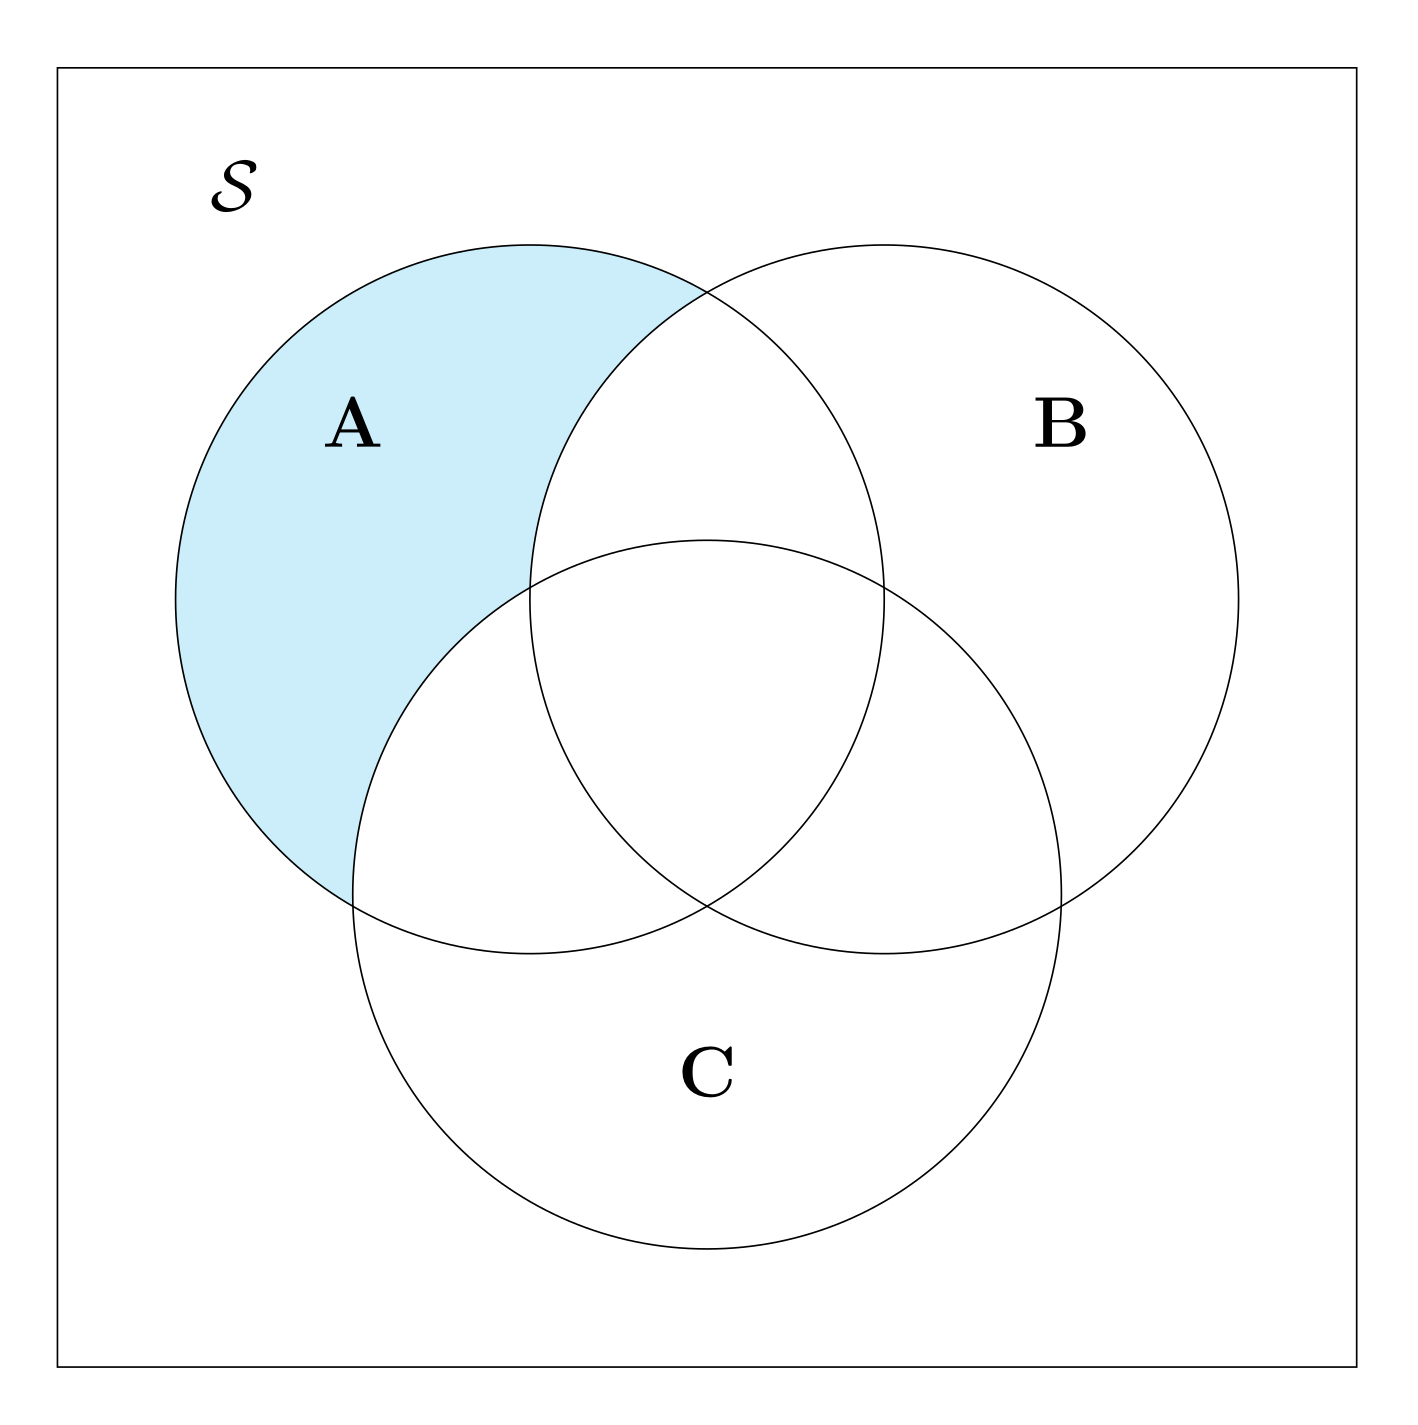
\includegraphics[width=\linewidth]{figures/w2-only-A.png}\\[3pt]
\small $A\setminus(B\cup C)$
\end{minipage}\hfill
\begin{minipage}[t]{0.31\linewidth}\centering

\includegraphics[width=\linewidth]{figures/w2-A-B-no-C.png}\\[3pt]
\small $(A\cap B)\setminus C$
\end{minipage}\hfill
\begin{minipage}[t]{0.31\linewidth}\centering

\includegraphics[width=\linewidth]{figures/w2-A-B-C.png}\\[3pt]
\small $A\cap B\cap C$
\end{minipage}
\end{center}

We now fill in the Venn diagram.

\notesfigure{figures/w2-commuters2-filled.png}

\item If we have already calculated out everything in each small category, it remains only to sum the values and divide by 100. This should give us $85/100 = 17/20$. Note that this is an example of the complement being easier to compute: adding up all the components is more tedious than just noticing that it must be $100 - 15 = 85$.

In more generality, we can use the inclusion-exclusion principle: in terms of sets $A$, $B$, and $C$, the probability may be computed by

\[
\begin{aligned}
\mathbb P(A \cup B \cup C)
  &= \mathbb P(A)+\mathbb P(B)+\mathbb P(C) \\
  &\quad -\mathbb P(A\cap B)-\mathbb P(A\cap C)-\mathbb P(B\cap C) \\
  &\quad +\mathbb P(A\cap B\cap C).
\end{aligned}
\]

Intuitively, we're adding everything included in all three sets, realizing that we're double counting and subtracting off overlaps, then realizing that we \emph{completely} removed the section where all \emph{three} overlap, and adding this last category back.

\item This probability rule does not require independence. It always holds, regardless of how the events are related to one another.

\end{enumerate}

\section*{Conditional Probability}

\blocktitle{Definition: Conditional Probability}

Let $\mathcal S$ be a sample space, and let $A$ and $B$ be events. Then if $\mathbb P(B) > 0$, the \emph{\textbf{conditional probability}} of $A$ given $B$ is defined as

\[
\mathbb P(A \,|\, B) = \frac{\mathbb P(A \cap B)}{\mathbb P(B)}.
\]

\blocktitle{Example: Delivery Alerts}

Suppose we have data on 400 deliveries that occurred in New York City. Let $L$ be the event that the delivery was late, and $F$ be the event that the delivery was flagged as "likely to be late" before the delivery occurred. Suppose we know that, for this group of deliveries,

\[
\mathbb P(L) = 0.20, \qquad \mathbb P(F \,|\, L) = 0.75, \qquad \mathbb P(F \,|\, L^c) = 0.25.
\]

\begin{enumerate}[label=\alph*.]

\item \begin{minipage}[t]{\linewidth}
Fill in the following table using the probabilities above.
\begin{center}
\small
\begin{tabular}{|l|c|c|c|}
\hline
 & \textbf{Late $L$} & \textbf{On time $L^c$} & \textbf{Total} \\ \hline
Flagged $F$ & \blank & \blank & \blank \\ \hline
Not flagged $F^c$ & \blank & \blank & \blank \\ \hline
\textbf{Total} & \blank & \blank & \textbf{400} \\ \hline
\end{tabular}
\end{center}
\end{minipage}

\item Compute $\mathbb P(F)$ and $\mathbb P(L \,|\, F)$. Suppose someone waiting on their package says, "An alerted delivery has a 75\% chance of being late." Is this statement accurate?

\end{enumerate}

\blocktitle{Solution}

\begin{enumerate}[label=\alph*.]

\item What can we fill in first? $\mathbb P(L)$ gives us that the "total" for $L$ (meaning both flagged and not flagged) makes up 20\% out of the 400 deliveries. Hence, we have that $.2 \cdot 400 = 80$ deliveries were late. Hence, 320 must have been on time. We can therefore fill in the "Total" row.

\begin{center}
\small
\begin{tabular}{|l|c|c|c|}
\hline
 & \textbf{Late $L$} & \textbf{On time $L^c$} & \textbf{Total} \\ \hline
Flagged $F$ & \blank & \blank & \blank \\ \hline
Not flagged $F^c$ & \blank & \blank & \blank \\ \hline
\textbf{Total} & 80 & 320 & \textbf{400} \\ \hline
\end{tabular}
\end{center}

What can we fill in next based on this information? The trick is to restrict our attention to specific rows and columns that the conditional probability information gives us. The second probability tells us that, out of everything in the $L$ (late) column, 75\% of them were flagged. Hence, we have that $.75 \cdot 80 = 60$ deliveries were flagged out of the 80 total that were late. Hence, $80 - 60 = 20$ of them must have not been flagged. We can therefore fill in the entire first column, $L$.

\begin{center}
\small
\begin{tabular}{|l|c|c|c|}
\hline
 & \textbf{Late $L$} & \textbf{On time $L^c$} & \textbf{Total} \\ \hline
Flagged $F$ & 60 & \blank & \blank \\ \hline
Not flagged $F^c$ & 20 & \blank & \blank \\ \hline
\textbf{Total} & 80 & 320 & \textbf{400} \\ \hline
\end{tabular}
\end{center}

We do the same thing using the third probability: we have that, out of the 320 deliveries that were not late, 25\% of them were flagged. We therefore have that $.25 \cdot 320 = 80$ were flagged despite ultimately being on time. Hence, $320 - 80 = 240$ were not late and were also not flagged. We therefore have the complete table.

\begin{center}
\small
\begin{tabular}{|l|c|c|c|}
\hline
 & \textbf{Late $L$} & \textbf{On time $L^c$} & \textbf{Total} \\ \hline
Flagged $F$ & 60 & 80 & 140 \\ \hline
Not flagged $F^c$ & 20 & 240 & 260 \\ \hline
\textbf{Total} & 80 & 320 & \textbf{400} \\ \hline
\end{tabular}
\end{center}

\item We now compute $\mathbb P(F)$ and $\mathbb P(L \,|\, F)$. Out of the $400$ deliveries total, we see that $140$ were flagged. Hence, $\mathbb P(F) = 140/400 = 7/20$. Next, out of the $140$ flagged deliveries, $60$ were actually late. Hence, $\mathbb P(L \,|\, F) = 60/140 = 3/7$. The person is wrong, then: they are saying that if a delivery is flagged, it has a probability of 0.75 of being late. In our formal notation, this is equivalent to claiming that

\[
\mathbb P(L \,|\, F) = 0.75.
\]

This is not what we computed. What the person actually should have said is, "If a delivery is late, there is a 0.75 chance that it had been flagged." This corresponds to the \emph{other} conditional probability,

\[
\mathbb P(F \,|\, L) = 0.75.
\]

\end{enumerate}

\clearpage
\blocktitle{Example: Training and Job Offers}

Let's consider a group of 200 people who are job-hunting. Out of the 200,

\begin{enumerate}[label=\roman*.]

\item 120 completed a training course.

\item 80 received a job offer during the following month.

\item 160 completed the training course, received a job offer, or both.

\end{enumerate}

For every person, we have recorded whether they completed the training course and whether they received a job offer. Suppose we select one person at random. Let $T$ be the event that the selected person completed the training course, and let $O$ be the event that they received a job offer.

\begin{enumerate}[label=\alph*.]

\item \begin{minipage}[t]{\linewidth}
Fill in the following table, including all row and column totals.
\begin{center}
\small
\begin{tabular}{|l|c|c|c|}
\hline
 & \textbf{Received an offer $O$} & \textbf{No offer $O^c$} & \textbf{Total} \\ \hline
Completed training $T$ & \blank & \blank & 120 \\ \hline
Did not complete training $T^c$ & \blank & \blank & \blank \\ \hline
\textbf{Total} & \textbf{80} & \blank & \textbf{200} \\ \hline
\end{tabular}
\end{center}
\end{minipage}

\item What is the probability that the selected person neither completed the training course nor received a job offer? What is the probability that \emph{exactly one} of these events occurred? You should first identify which cells you will need for your calculation.

\item Compute $\mathbb P(O \,|\, T)$ and $\mathbb P(T \,|\, O)$. What do these probabilities each mean?

\item Are $T$ and $O$ independent? How does this help us answer the question of whether a person who completed the training has a higher chance of getting an offer?

\end{enumerate}

\blocktitle{Solution}

\begin{enumerate}[label=\alph*.]

  
\item Let's fill in the two remaining "Total" cells first.

\begin{center}
\small
\begin{tabular}{|l|c|c|c|}
\hline
 & \textbf{Received an offer $O$} & \textbf{No offer $O^c$} & \textbf{Total} \\ \hline
Completed training $T$ & \blank & \blank & 120 \\ \hline
Did not complete training $T^c$ & \blank & \blank & 80 \\ \hline
\textbf{Total} & \textbf{80} & 120 & \textbf{200} \\ \hline
\end{tabular}
\end{center}

To fill in the remaining cells, we will need to utilize the fact that 160 people completed the training course, received a job offer, or both. The cells in question are "$T$ and $O$", "$T^c$ and $O$", and "$T$ and $O^c$". But wait! There's something we should notice: the only cell remaining is $T^c \cap O^c$, which is the cell containing the individuals who neither completed the training course nor received an offer. We can therefore fill that in, which must be $200 - 160 = 40$.

\begin{center}
\small
\begin{tabular}{|l|c|c|c|}
\hline
 & \textbf{Received an offer $O$} & \textbf{No offer $O^c$} & \textbf{Total} \\ \hline
Completed training $T$ & \blank & \blank & 120 \\ \hline
Did not complete training $T^c$ & \blank & 40 & 80 \\ \hline
\textbf{Total} & \textbf{80} & 120 & \textbf{200} \\ \hline
\end{tabular}
\end{center}

We can now complete the table.

\begin{center}
\small
\begin{tabular}{|l|c|c|c|}
\hline
 & \textbf{Received an offer $O$} & \textbf{No offer $O^c$} & \textbf{Total} \\ \hline
Completed training $T$ & 40 & 80 & 120 \\ \hline
Did not complete training $T^c$ & 40 & 40 & 80 \\ \hline
\textbf{Total} & \textbf{80} & 120 & \textbf{200} \\ \hline
\end{tabular}
\end{center}

\item The probability that the selected person neither completed the training course nor received a job offer is $40/200 = 1/5$. This is computed using the cell containing individuals who did not do the training course or receive an offer. The probability that exactly one of events $T$ and $O$ occurred can be computed as follows: we first count the individuals who either completed the training course and did not receive an offer or did not complete the training course but did receive an offer. Summing these two cells gives us $40 + 80 = 120$ individuals. The probability is therefore $120/200 = 3/5$.

  
\item Next, we compute $\mathbb P(O \,|\, T)$ and $\mathbb P(T \,|\, O)$. Restricting to the first row, which has 120 individuals, we have that 40 of them received an offer, making $\mathbb P(O \,|\, T) = 1/3$. Restricting to the first column, which contains 80 individuals, we see that 40 of them completed the training. Hence, $\mathbb P(T \,|\, O) = 1/2$. The former conditional probability is the chance that the applicant receives an offer given that they completed a training course. The latter represents the chance that the applicant had completed training given that they received an offer.

  
\item $T$ and $O$ are \emph{not} independent. The probability of receiving an offer is $80/200 = 2/5$. The probability of the applicant having received an offer given that they completed the training course is, as calculated above, $1/3$, which is smaller than $2/5$. Thus, knowing that the applicant completed a training course "changes" the probability. An applicant who completed the training course is less likely to have received an offer than one who did not.

\end{enumerate}

\clearpage
\section*{Independence}

\blocktitle{Definition: Independent Events}

Let $\mathcal S$ be a sample space, and let $A$ and $B$ be events. Then $A$ and $B$ are \emph{\textbf{independent}}, denoted $A \perp B$, if

\[
\mathbb P(A \cap B) = \mathbb P(A) \cdot \mathbb P(B).
\]

\blocktitle{Definition: Disjoint Events}

Let $\mathcal S$ be a sample space, and let $A$ and $B$ be events. Then $A$ and $B$ are \emph{\textbf{disjoint}} if

\[
A \cap B = \emptyset.
\]

\blocktitle{Definition: Pairwise Independence}

Let $A_1, A_2, \ldots, A_n$ be events. The events are \emph{pairwise independent} if any two distinct events are independent: for every $i \ne j$,

\[
\mathbb P(A_i \cap A_j) = \mathbb P(A_i) \cdot \mathbb P(A_j).
\]

\blocktitle{Definition: Mutual Independence}

Let $A_1, A_2, \ldots, A_n$ be events. The events are \emph{mutually independent} if, for every subset of distinct events $A_{k_1}, A_{k_2}, \ldots, A_{k_\ell}$, with $2 \leq \ell \leq n$,

\[
\mathbb P(A_{k_1} \cap A_{k_2} \cap \cdots \cap A_{k_\ell}) = \mathbb P(A_{k_1}) \cdot \mathbb P(A_{k_2}) \cdots \mathbb P(A_{k_\ell}).
\]

\blocktitle{Example: Two Dice Rolls}

Suppose we have two fair six-sided dice, and we independently roll each of them. Let us define four events: let $A_1$ be the event that die 1 rolls an odd number. Let $A_2$ be the event that die 1 rolls an even number. Let $A_3$ be the event that die 2 rolls an odd number. Let $A_4$ be the event that the sum of the numbers on the two dice is odd.

\begin{enumerate}[label=\alph*.]

  
\item Are $A_1$ and $A_2$ independent? Are they disjoint? Are $A_1$ and $A_3$ independent? Are $A_2$ and $A_3$?

  
\item Are $A_1$ and $A_4$ independent? You might need to calculate out the conditional probabilities.

  
\item Are $A_2$, $A_3$, and $A_4$ pairwise independent? Are they mutually independent?

\end{enumerate}

\clearpage
\blocktitle{Solution}

\begin{enumerate}[label=\alph*.]

  
\item $A_1$ and $A_2$ are clearly not independent. They are disjoint: if I know that $A_1$ has occurred, that means that the first die rolled an odd number, and therefore cannot have rolled an even number. $A_1$ and $A_3$ are independent: the outcome of one dice roll does not impact the outcome of another. Similarly, $A_2$ and $A_3$ are also independent, as they are events for two independently rolled dice.

  
\item $A_1$ and $A_4$ are indeed independent. We can directly and explicitly count the outcomes. Let's first calculate what the probabilities for the two events themselves are.

What is the probability that die 1 rolls an odd number? Three out of six equally probable outcomes are odd, so the probability is $1/2$. This is true for die 2 as well.

What is the probability that the sum of the two numbers is odd? If both numbers are even or both numbers are odd, the sum is even. These two outcomes both have probability $(1/2) \cdot (1/2) = 1/4$. Summing them gives $1/2$ again. Then we already know the probability that the sum is an odd number is $1/2$, but let's compute it anyway: if the first number is even and the second is odd, then we have that the sum is odd. Similarly, if the first number is odd and the second is even, we also have that the sum is odd. Both of these also have a probability of $(1/2) \cdot (1/2) = 1/4$, and summing them also gives $1/2$.

Now we calculate the conditional probability. Suppose that $A_1$ has occurred, meaning the first die rolled an odd number. What is the probability that the sum is odd? In order for $A_4$ to occur, $A_3^c$ must occur, meaning the second die needs to be even. This has probability $1/2$ of occurring. Therefore, the conditional probability $\mathbb P(A_4 \,|\, A_1) = 1/2 = \mathbb P(A_4)$.

Similarly, one can compute that $\mathbb P(A_1 \,|\, A_4) = \mathbb P(A_1)$. We have that $\mathbb P(A_1) = 1/2$. Knowing that the sum is odd gives us that either die 1 rolled an even number and die 2 odd, or the other way around. These two events have equal probability, so we have that $\mathbb P(A_1 \,|\, A_4) = 1/2$ as well. Hence, $A_1 \perp A_4$.

  
\item We can easily compute that $A_2 \perp A_4$ and $A_3 \perp A_4$ in exactly the same way as above. $A_2$ is also independent of $A_3$, as they concern the outcomes of independent dice rolls. Hence, every pair we can choose from $A_2, A_3, A_4$ is independent, and we may conclude that this collection of events is pairwise independent.

Are they mutually independent? It turns out that they are not. Suppose we know that events $A_2$ and $A_3$ both occurred. That means that $A_4$ \emph{must} have occurred: if we already know that die 1 was even and die 2 was odd, then the sum must be odd. Therefore, while $\mathbb P(A_4) = 1/2$, we have that $\mathbb P(A_4 \,|\, A_2, A_3) = 1$. Similarly, if we know that event $A_2$ occurred but that event $A_3$ did \emph{not} occur, we know that the sum must be even, and $A_4$ cannot occur. Therefore, the events are not mutually independent.

\end{enumerate}

\end{document}
